\documentclass[10pt]{article}
\usepackage[spanish]{babel}
\usepackage[utf8]{inputenc}
\usepackage[T1]{fontenc}
\usepackage[margin=1.2cm, footskip=0.45cm]{geometry}
\usepackage{graphicx}
\usepackage{amsmath}
\usepackage{booktabs}
\usepackage{float}
\usepackage{tabularx}
\usepackage{caption}
\usepackage{subcaption}
\usepackage{hyperref}

\hypersetup{colorlinks=true, linkcolor=black, urlcolor=blue, citecolor=black}
\setlength{\parindent}{0pt}
\setlength{\parskip}{0.23em}
\setlength{\tabcolsep}{4pt}
\renewcommand{\arraystretch}{1.05}
\captionsetup{font=small, labelfont=bf}

\title{\textbf{Proyecto 2 - Freesound Audio Tagging}\\Taller de Aprendizaje Automático}
\author{Luciana García \and Santiago Márquez \and Santiago Rodríguez}
\date{\today}

\begin{document}
\maketitle

\section{Introducción}
\subsection{Problema y enfoque}
El objetivo del proyecto es identificar automáticamente las fuentes sonoras
presentes en una grabación. A diferencia de una clasificación tradicional de una
sola clase, Freesound Audio Tagging 2019 es un problema \textit{multi-label}: un
audio puede contener más de una etiqueta, y la salida esperada por Kaggle es una
probabilidad para cada una de las 80 clases. Por este motivo, el modelo se
entrena con salidas sigmoides independientes y se evalúa con \textit{label-weighted
label-ranking average precision} (lwlrap), una métrica de ranking que premia que
las clases correctas queden altas en la lista de probabilidades de cada audio.

La solución final se apoya en una hipótesis central: para audio ambiental, la
estructura tiempo-frecuencia del espectrograma es más informativa que un resumen
tabular global. Por eso el camino de trabajo fue pasar de estadísticas simples
de log-mel a redes convolucionales sobre imágenes log-mel, y luego combinar tres
ramas que miran el mismo fenómeno con sesgos distintos. La entrega oficial es:

\begin{center}
\texttt{0.25 H100 + 0.375 G100 + 0.375 F100}
\end{center}

donde \texttt{H100} es una CNN separable-residual con cabeza densa, \texttt{G100}
agrega normalización global por banda Mel y una cabeza temporal BiGRU, y
\texttt{F100} usa una ventana temporal más larga de 1024 frames. El score privado
de Kaggle asociado a este CSV es \textbf{0.67126}.

\subsection{Metodología general}
El trabajo se organizó en cuatro etapas. Primero se analizó el dataset, el
desbalance y la métrica. Luego se construyeron caches reproducibles de
representaciones log-mel para evitar recalcular audio crudo en cada
experimento. En la tercera etapa se compararon familias de modelos y
arquitecturas CNN. Finalmente se fijó un sistema de tres ramas a 100 épocas y se
evaluaron variantes de ponderación y bagging. La decisión final no tomó el mayor
score absoluto, sino el mejor equilibrio entre desempeño, simplicidad y defensa
conceptual.

\section{Datos, métrica y riesgos}
\subsection{Estructura del dataset}
Se trabajó con tres archivos principales: \texttt{train\_curated.csv},
\texttt{train\_noisy.csv} y \texttt{sample\_submission.csv}. El conjunto curado
tiene etiquetas más confiables y fue la base del entrenamiento final; el conjunto
ruidoso se analizó como fuente posible, pero no se concatenó directamente porque
en experimentos tempranos degradó la validación curada. Además se descartaron
seis archivos conocidos como problemáticos antes de entrenar.

\begin{table}[H]
\centering
\small
\begin{tabular}{@{}lrrr@{}}
\toprule
Split & Filas & Archivos únicos & Etiquetas promedio/audio \\
\midrule
train\_curated & 4970 & 4970 & 1.157 \\
train\_noisy & 19815 & 19815 & 1.211 \\
test & 3361 & 3361 & -- \\
\bottomrule
\end{tabular}
\caption{Tamaño de los conjuntos disponibles. El modelo final entrena sobre el
conjunto curado y genera probabilidades para los 3361 audios de test.}
\label{tab:splits}
\end{table}

Hay 80 clases y 5752 asignaciones de etiquetas en \texttt{train\_curated}. La
mediana de ejemplos por clase es 75, el mínimo observado es 47 y tres clases
tienen menos de 50 ejemplos. El desbalance no es extremo por clase individual,
pero sí hay una cola de clases raras y una estructura multi-label que hace que
la exactitud no sea una métrica adecuada.

\begin{figure}[H]
\centering
\begin{subfigure}{0.44\textwidth}
\centering
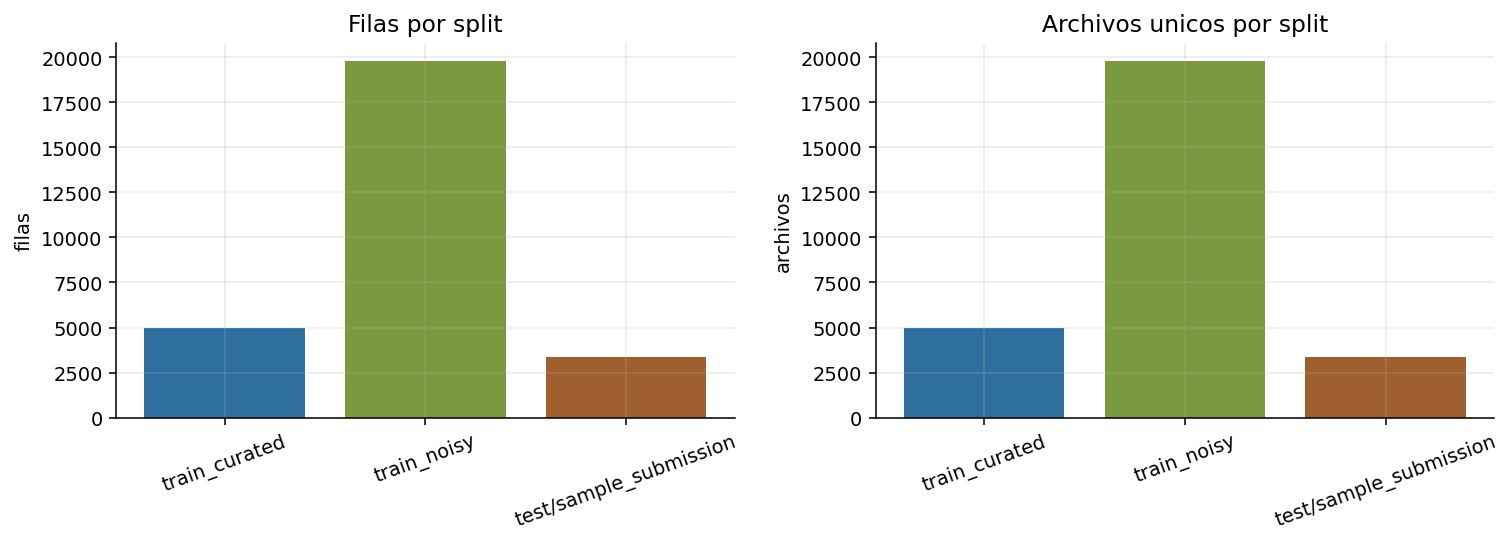
\includegraphics[width=\linewidth]{img/fig_split_sizes.png}
\caption{Tamaño de splits.}
\end{subfigure}
\hfill
\begin{subfigure}{0.53\textwidth}
\centering
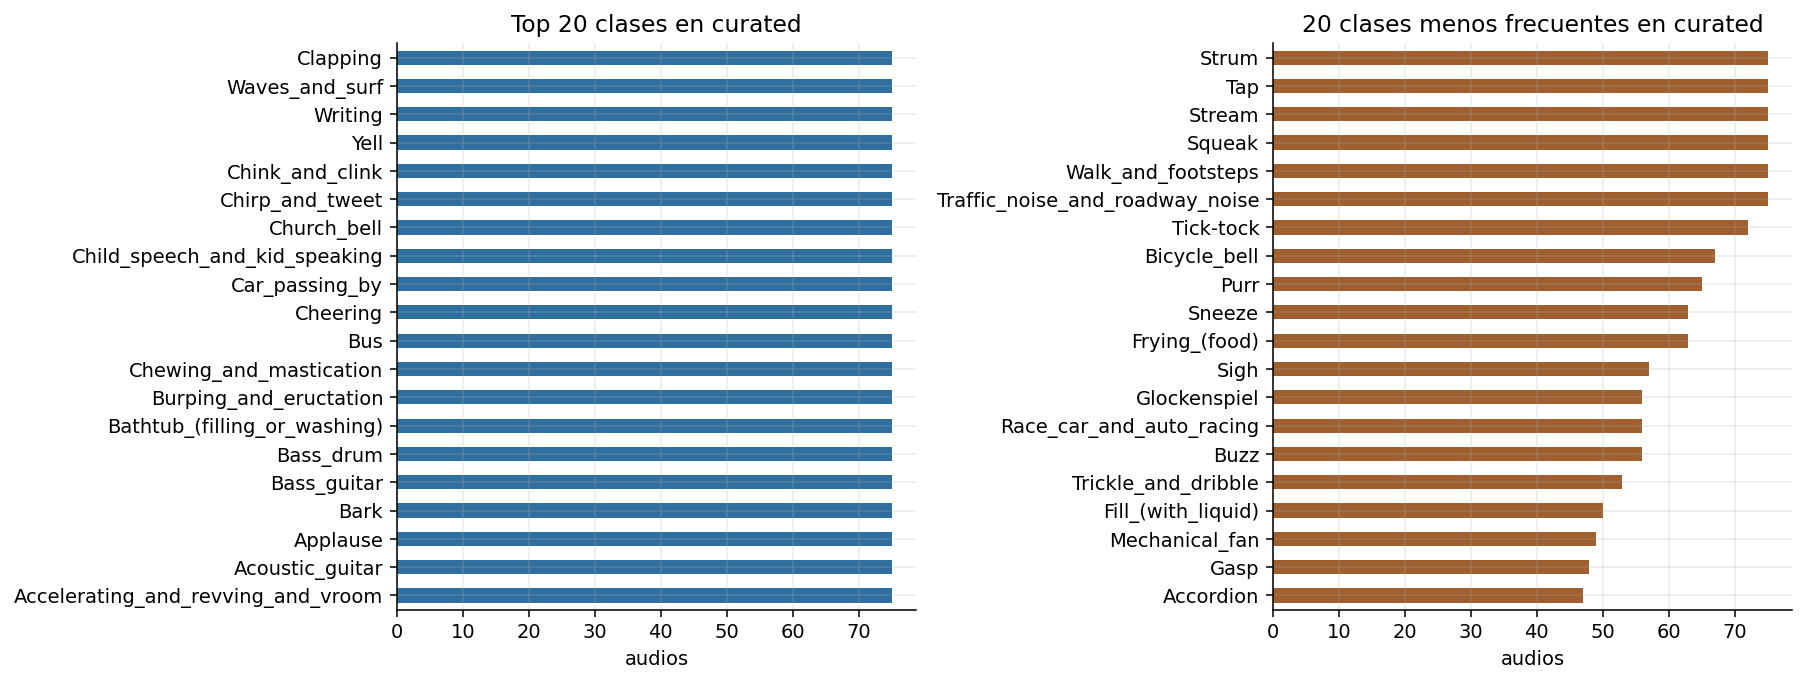
\includegraphics[width=\linewidth]{img/fig_label_frequency.png}
\caption{Clases frecuentes y raras.}
\end{subfigure}
\caption{Estructura de datos y desbalance de etiquetas en el conjunto curado.}
\label{fig:data}
\end{figure}

\subsection{Métrica lwlrap}
Kaggle evalúa con lwlrap. Para cada audio se ordenan las clases por score y se
mide la precisión acumulada en las posiciones donde aparecen clases verdaderas.
Luego se promedia ponderando por la frecuencia de cada clase. Esto favorece
modelos que ordenan bien las clases relevantes incluso cuando las probabilidades
no están perfectamente calibradas:

\begin{equation}
\mathrm{lwlrap} = \sum_{c=1}^{C} w_c \cdot
\frac{1}{N_c}\sum_{i: y_{ic}=1} \mathrm{precision}_{i,c}.
\end{equation}

Esta métrica justificó trabajar con blends de probabilidades: si dos ramas
cometen errores distintos, el promedio puede mejorar el ranking final aunque no
cambie la arquitectura interna de cada componente.

\section{Representación de audio}
\subsection{De WAV a log-mel}
El preprocesamiento común convierte cada audio en una imagen log-mel:

\begin{center}
\texttt{.wav -> mono -> 44.1 kHz -> MelSpectrogram -> log/dB -> crop/pad -> normalización}
\end{center}

Se usaron 128 bandas Mel. El eje horizontal contiene frames de tiempo; por
ejemplo, una entrada \texttt{128 x 512} significa 128 bandas de frecuencia
perceptual y 512 pasos temporales. Esta representación conserva patrones como
ataques, bandas tonales, ruido broadband y repeticiones, que se pierden al
colapsar el espectrograma en estadísticas globales.

\begin{figure}[H]
\centering
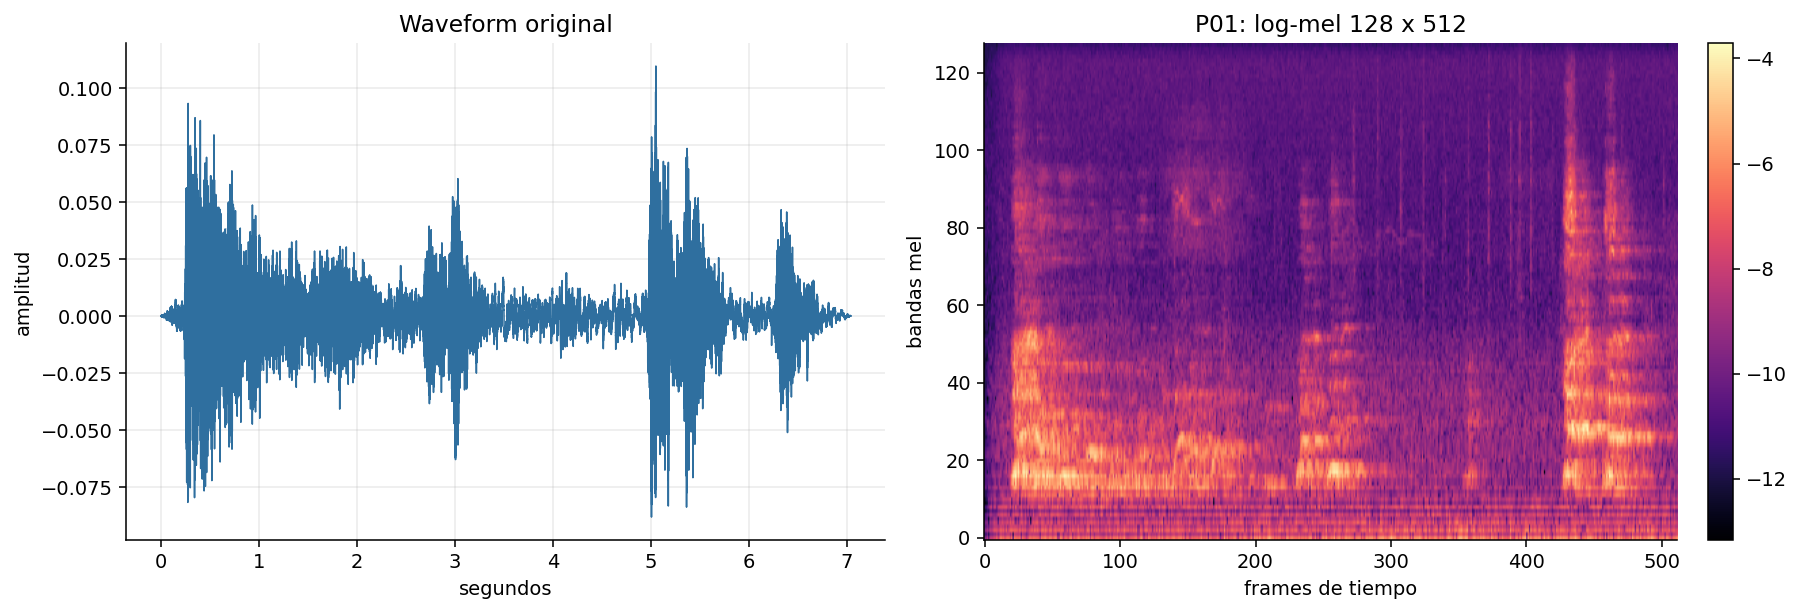
\includegraphics[width=0.82\textwidth]{img/fig_waveform_logmel.png}
\caption{Ejemplo del pasaje desde forma de onda a imagen log-mel. La CNN opera
sobre esta estructura tiempo-frecuencia.}
\label{fig:logmel}
\end{figure}

\subsection{Variantes de preprocesamiento}
Como resume la Tabla~\ref{tab:preproc}, se probaron tres niveles de representación. \texttt{P00} resume el log-mel en
features tabulares y sirve como baseline barato. \texttt{P01} conserva la imagen
\texttt{128 x 512}, permitiendo entrenar CNNs. \texttt{P02} agrega dos ideas que
terminan en el final: normalización global por banda Mel y ventana temporal
\texttt{128 x 1024}.

\begin{table}[H]
\centering
\small
\begin{tabularx}{\textwidth}{@{}lXrl@{}}
\toprule
Pipeline & Idea & Private LB & Decisión \\
\midrule
P00 & Estadísticas tabulares de log-mel; pierde el eje temporal. & 0.37607 & baseline \\
P01 & Imagen log-mel \texttt{128 x 512} para CNN. & 0.52257 & mantener \\
P01 + entrenamiento & He, scheduler, BatchNorm, dropout y cabeza densa. & 0.64665 & mantener \\
P02 global-mel & Normalización global por banda Mel. & 0.66561 & mantener \\
P02 f1024 & Contexto temporal de 1024 frames. & 0.67025 & evidencia pre-final \\
\bottomrule
\end{tabularx}
\caption{Evolución de las representaciones. El salto grande ocurre al conservar
la estructura tiempo-frecuencia para CNNs.}
\label{tab:preproc}
\end{table}

\begin{figure}[H]
\centering
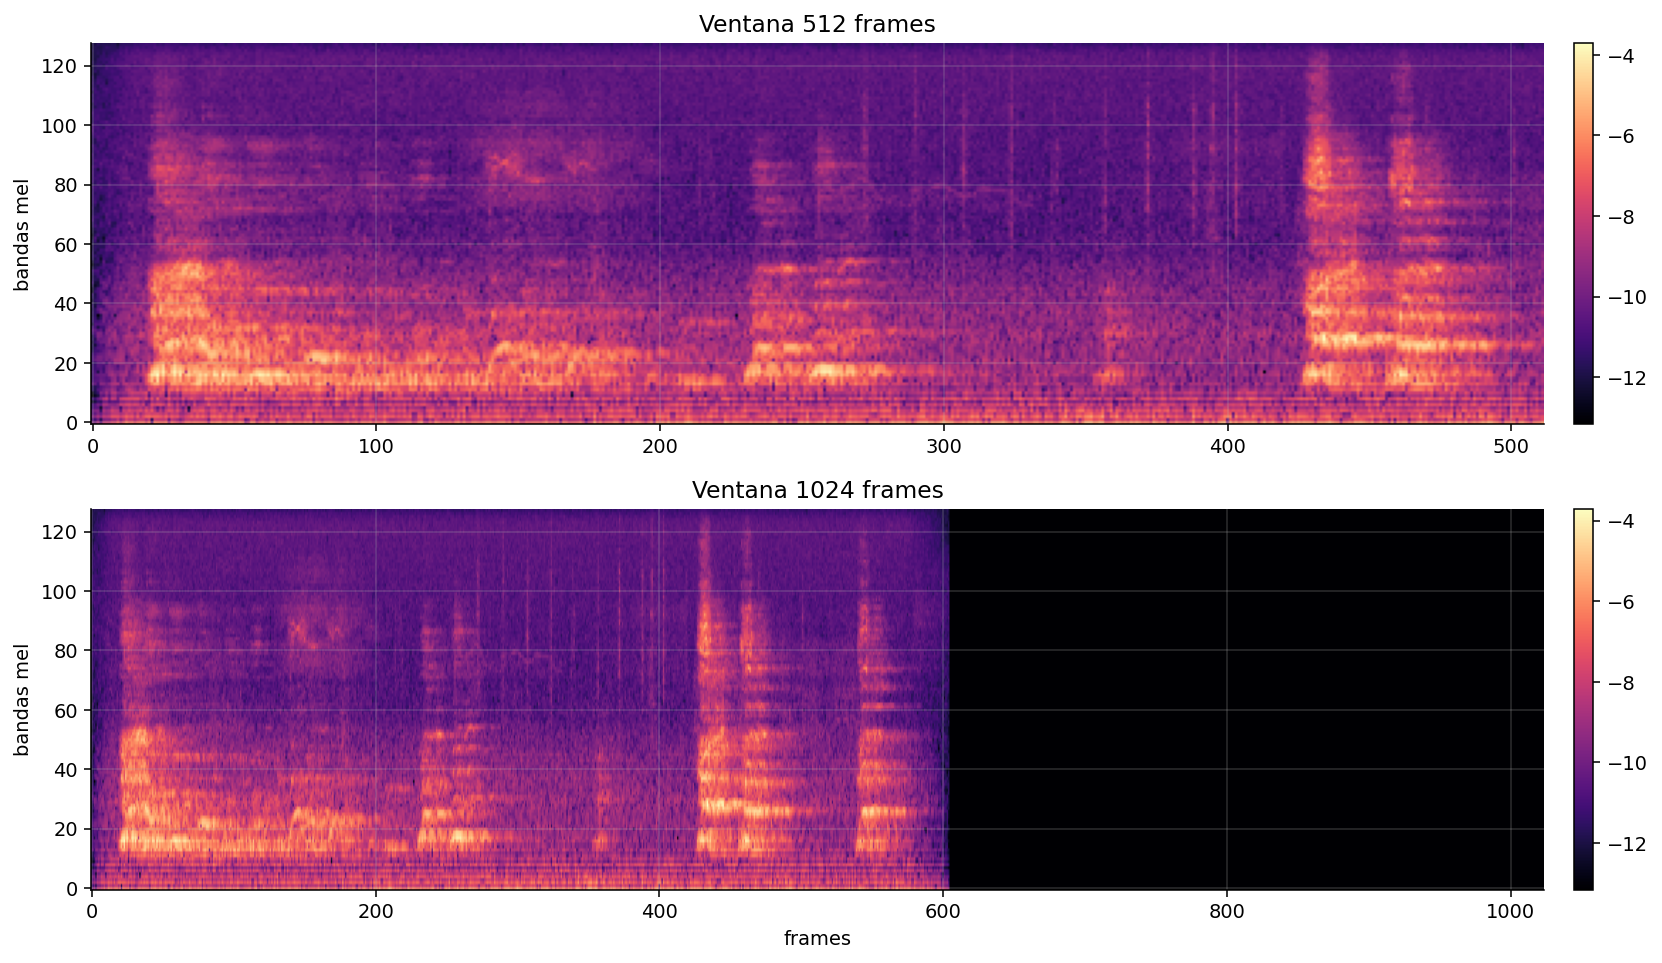
\includegraphics[width=0.78\textwidth]{img/fig_f512_f1024.png}
\caption{Comparación conceptual entre ventana de 512 frames y ventana de 1024
frames. La segunda conserva más contexto temporal para eventos largos.}
\label{fig:f1024}
\end{figure}

\section{Modelos y experimentación}
\subsection{Hipótesis evaluadas}
La experimentación se guió por hipótesis concretas, cuyo impacto acumulado se
ve en la Figura~\ref{fig:ladder}:

\begin{itemize}
\item \textbf{H1:} resumir log-mel en estadísticas no alcanza, porque colapsa el
tiempo. La mejora de 0.37607 a 0.52257 al usar CNN confirma esta hipótesis.
\item \textbf{H2:} mejorar entrenamiento y regularización de CNNs puede aportar
tanto como cambiar arquitectura. La etapa con He, scheduler, BatchNorm, dropout
y cabeza densa sube hasta 0.64665.
\item \textbf{H3:} ramas con sesgos distintos producen errores complementarios.
La normalización global Mel y la rama temporal \texttt{f1024} mejoran los blends.
\item \textbf{H4:} más complejidad no siempre debe entrar al final. Bagging de
ramas temporales alcanza 0.67674, pero agrega modelos internos y reduce claridad.
\end{itemize}

\begin{figure}[H]
\centering
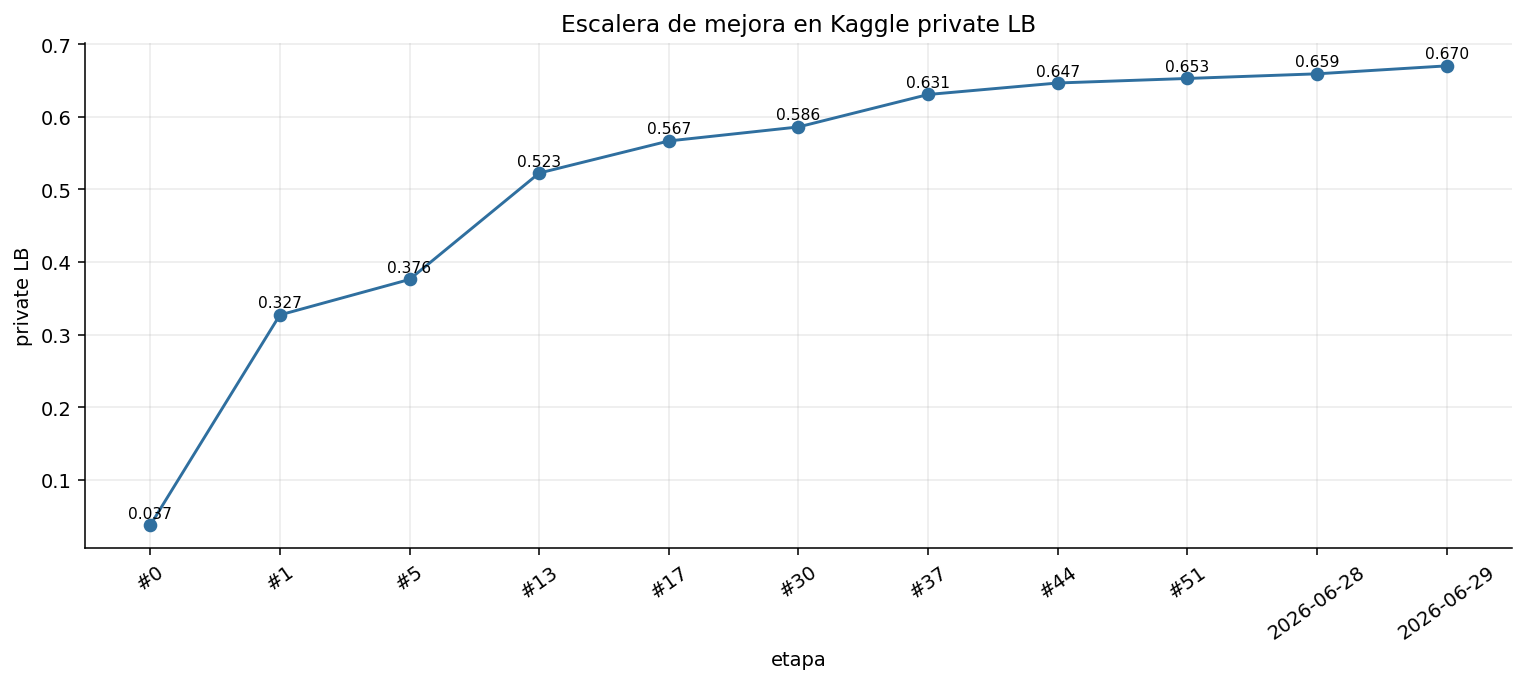
\includegraphics[width=0.84\textwidth]{img/fig_private_lb_ladder.png}
\caption{Escalera de mejoras en private leaderboard. Cada salto corresponde a
una decisión experimental documentada.}
\label{fig:ladder}
\end{figure}

\subsection{Arquitecturas comparadas}
La comparación incluyó al menos dos familias CNN sobre espectrogramas. La CNN
log-mel inicial preserva la imagen \texttt{128 x 512} pero usa bloques más
simples. La familia final usa bloques separables-residuales: primero una
convolución depthwise por canal, luego una convolución \texttt{1 x 1} para
mezclar canales, BatchNorm y activación. Esta variante es más eficiente y
estable, y permitió construir una rama fuerte con cabeza densa.

También se evaluó una variante de transferencia con ResNet50 congelada desde
ImageNet. El resultado individual fue débil para usarlo como modelo principal,
pero aportó diversidad en blends históricos. Se mantuvo como evidencia de
experimentación y no como componente final. Con datos ruidosos ocurrió algo
similar: la concatenación directa de \texttt{train\_noisy} empeoró la validación
curada, por lo que se descartó para el final y se dejó como línea futura para
preentrenamiento o filtrado.

\begin{table}[H]
\centering
\scriptsize
\begin{tabularx}{\textwidth}{@{}lXlX@{}}
\toprule
Prueba & Evidencia & Decisión & Lectura \\
\midrule
Transfer ResNet50/ImageNet & débil individual; útil solo como diversidad en
blend & no final & la transferencia visual no trasladó suficiente semántica
de audio \\
Concatenar \texttt{train\_noisy} & validación curada cae a 0.3567 & descartar &
el ruido de etiquetas requiere filtrado o preentrenamiento, no mezcla directa \\
Time reverse / contraste & valid lwlrap 0.764--0.771 contra 0.808 de la rama
headsep comparable & descartar & algunas augmentations no preservan bien la
semántica sonora \\
CNN separable-residual & valid lwlrap 0.8078 y Private LB 0.65289 & mantener &
mejora capacidad sin perder una explicación simple \\
\bottomrule
\end{tabularx}
\caption{Pruebas asociadas a requisitos de la consigna que no entraron
directamente al modelo final.}
\label{tab:reqtests}
\end{table}

\section{Modelo final}
\subsection{Tres ramas complementarias}
La entrega oficial combina tres componentes entrenados a 100 épocas con semilla
42. Las tres usan log-mel, pero no son redundantes.

\begin{table}[H]
\centering
\scriptsize
\begin{tabularx}{\textwidth}{@{}lcllX@{}}
\toprule
Rama & Peso & Entrada & Normalización & Rol \\
\midrule
\texttt{separable\_headsep} & 0.25 & \texttt{128 x 512} & por clip &
patrones locales tiempo-frecuencia con CNN separable-residual y cabeza densa \\
\texttt{globalmel\_sep\_temporal} & 0.375 & \texttt{128 x 512} & global Mel &
escala estable por banda y evolución temporal con BiGRU \\
\texttt{sep\_temporal\_f1024} & 0.375 & \texttt{128 x 1024} & por clip &
contexto temporal largo con CNN separable-residual y BiGRU \\
\bottomrule
\end{tabularx}
\caption{Componentes del blend final. Los pesos suman 1 y dan mayor peso conjunto
a las ramas temporales.}
\label{tab:components}
\end{table}

La rama \texttt{separable\_headsep} termina en pooling global y una cabeza densa,
por lo que resume la activación espacial final. Las ramas temporales no colapsan
tan pronto el eje de tiempo: la CNN extrae mapas tiempo-frecuencia y una BiGRU
bidireccional modela la secuencia resultante antes de clasificar.

\begin{figure}[H]
\centering
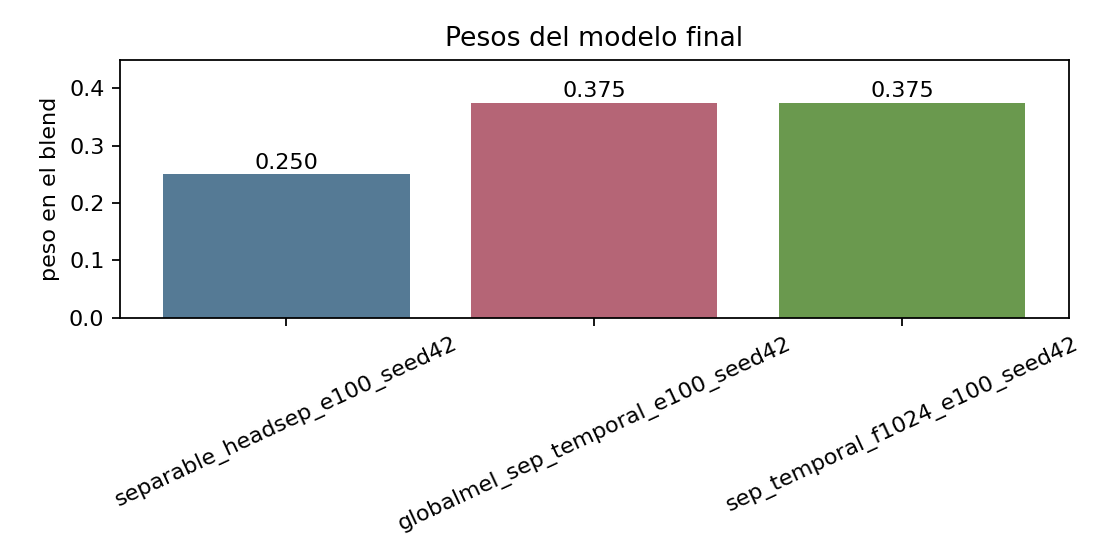
\includegraphics[width=0.62\textwidth]{img/fig_component_weights.png}
\caption{Pesos del blend final. La reponderación baja la rama puramente
convolucional y sube las dos ramas temporales.}
\label{fig:weights}
\end{figure}

\subsection{Regularización e hiperparámetros}
La regularización no depende de una sola técnica. Las tres ramas usan
\texttt{head\_dropout=0.3} y BatchNorm en los bloques convolucionales. Durante
entrenamiento se aplica SpecAugment sobre el log-mel: corrimiento temporal,
máscara temporal y máscara de frecuencia. Las ramas temporales usan AdamW con
\texttt{weight\_decay=1e-4}; la rama \texttt{headsep} usa Adam, por lo que en el
trainer actual no recibe L2 efectiva. Además, la pérdida es
\texttt{BCEWithLogitsLoss} con \texttt{pos\_weight} calculado desde el conjunto
curado para compensar desbalance por clase.

Se dejaron apagadas opciones que agregaban complejidad sin evidencia suficiente:
\texttt{block\_dropout=0}, \texttt{early\_stopping=0}, inversión temporal y
cambio aleatorio de contraste. La configuración final es por lo tanto simple de
explicar: tres ramas, 100 épocas, augmentation controlada y blend lineal.

Para controlar subajuste y sobreajuste se observó simultáneamente pérdida de
entrenamiento, lwlrap de validación y leaderboard. En la rama separable-residual
con cabeza densa, por ejemplo, la pérdida bajó de 0.601 a 0.023 y la validación
subió hasta 0.8078 alrededor de la época 56; luego osciló levemente, señal de
que seguir entrenando esa corrida ya aportaba poco al holdout. En las corridas
finales se priorizó \textit{full-train} a 100 épocas porque la evidencia de
Kaggle de la Tabla~\ref{tab:finalexp} mostró mejora al usar toda la data curada
y no únicamente el split local.

\section{Resultados y selección final}
La ronda a 100 épocas mostró que la arquitectura conceptual seguía mejorando al
entrenar más. El sistema de tres ramas con pesos iguales alcanzó 0.67055, y la
reponderación \texttt{0.25/0.375/0.375} subió a 0.67126. Luego se probaron
baggings internos sobre ramas temporales: el mejor llegó a 0.67674, pero se
descartó como entrega principal por depender de más modelos y ser menos directo
para defender en el tiempo disponible. La diferencia a favor del mejor
experimento es 0.00548, pero la entrega oficial mantiene tres componentes
físicos no baggeados y una fórmula de pesos simple.

\begin{table}[H]
\centering
\small
\begin{tabularx}{\textwidth}{@{}lclX@{}}
\toprule
Candidato & Private LB & Estado & Razón \\
\midrule
3-way original & 0.66649 & referencia & tres ramas previas con pesos iguales \\
3-way e100 equal & 0.67055 & mantiene & misma idea entrenada a 100 épocas \\
3-way e100 weighted & 0.67126 & final oficial & tres componentes físicos y pesos simples \\
globalmel bagged & 0.67528 & experimento & mejora parcial con bagging interno \\
globalmel + f1024 bagged & 0.67674 & mejor score & más complejo; no se elige como entrega \\
\bottomrule
\end{tabularx}
\caption{Comparación de variantes alrededor del modelo final.}
\label{tab:finalexp}
\end{table}

\begin{figure}[H]
\centering
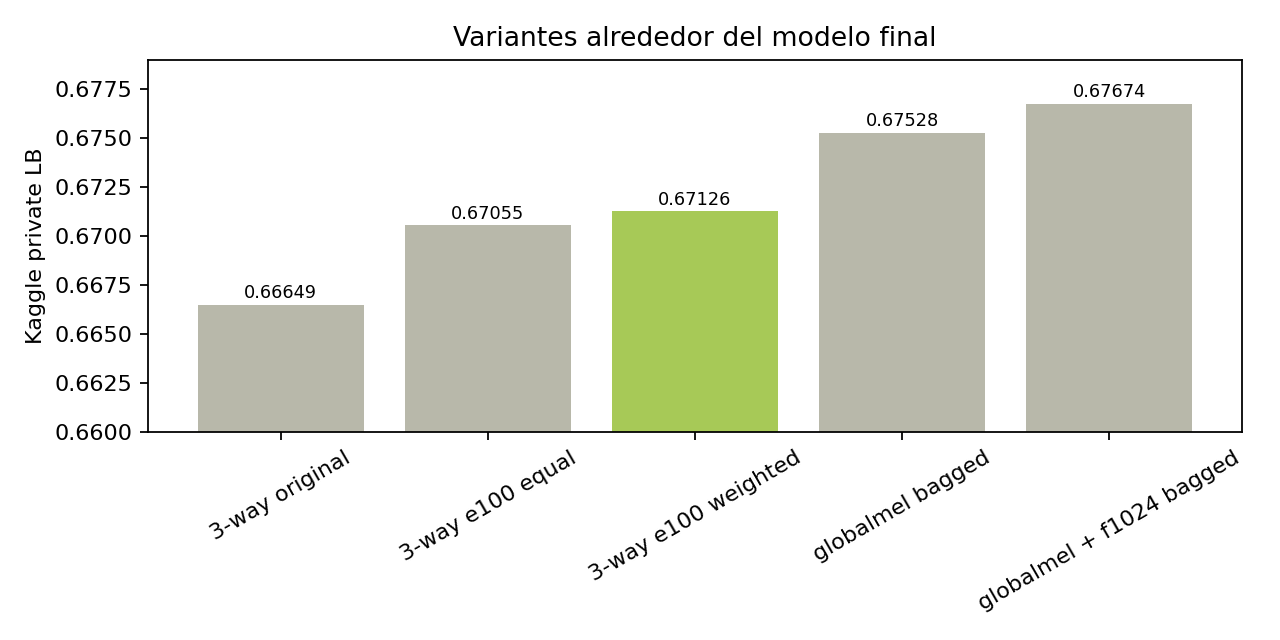
\includegraphics[width=0.78\textwidth]{img/fig_final_experiments.png}
\caption{Experimentos finales. El mejor score absoluto queda documentado, pero la
entrega oficial prioriza trazabilidad y simplicidad.}
\label{fig:finalexp}
\end{figure}

\section{Entrega reproducible}
El código de entrega queda en \texttt{proyecto\_actual/codigo/}. El notebook
\texttt{pipeline\_final\_taller\_2.ipynb} recompone el blend, valida columnas,
orden de archivos, rango de probabilidades y hash SHA-256 del CSV oficial:

\begin{center}
\texttt{4247ab9ff6398fbb1b6af223629d004265e27bb6cbccabf53ec4969a96c61cab}
\end{center}

El mismo notebook contiene los comandos pesados para reconstruir caches log-mel
y entrenar las tres ramas si se activa \texttt{RUN\_HEAVY\_STEPS=True}. En modo
entrega se ejecuta rápido usando los artefactos oficiales ya generados, lo que
facilita verificar la submission sin exigir una GPU.

\subsection{Lectura de predicciones de validación}
Para interpretar valoraciones del clasificador se revisaron ejemplos de un
holdout de la rama separable-temporal. La Tabla~\ref{tab:interpretacion} muestra
dos casos: uno donde las clases verdaderas aparecen arriba del ranking y otro
donde el modelo confunde el evento con fuentes acústicamente cercanas o
espurias.

\begin{table}[H]
\centering
\scriptsize
\begin{tabularx}{\textwidth}{@{}lX X X@{}}
\toprule
Audio & Etiquetas reales & Top-5 predicho & Lectura \\
\midrule
\texttt{dabca820.wav} & Applause, Crowd, Cheering &
Applause 0.998; Cheering 0.988; Crowd 0.981; Clapping 0.056; Frying 0.023 &
ranking correcto: las tres etiquetas reales quedan primeras y con alta
confianza \\
\texttt{765a95d3.wav} & Car passing by, Traffic noise &
Motorcycle 0.908; Revving 0.854; Microwave 0.448; Race car 0.270; Bus 0.128 &
error interpretable: activa clases de motores y tránsito, pero no las etiquetas
exactas esperadas \\
\bottomrule
\end{tabularx}
\caption{Ejemplos de interpretación de scores en validación.}
\label{tab:interpretacion}
\end{table}

\section{Conclusiones}
El resultado principal del proyecto es que la representación importa tanto como
la arquitectura. El salto más claro aparece al pasar de estadísticas globales de
log-mel a imágenes log-mel para CNNs. Luego, la mejora sostenida viene de
agregar diversidad controlada: normalización global por banda Mel, lectura
temporal con BiGRU y mayor contexto temporal. La submission oficial no es el
máximo score exploratorio, sino la variante más defendible: conserva tres
componentes conceptuales, evita bagging interno adicional y alcanza un private
LB competitivo de 0.67126.

Como trabajo futuro, el uso de \texttt{train\_noisy} podría retomarse con una
estrategia más cuidadosa, por ejemplo preentrenamiento con etiquetas débiles,
filtrado por confianza o fine-tuning progresivo. También sería natural mejorar
interpretabilidad visual revisando ejemplos de validación donde cada rama
asigna alta probabilidad a clases distintas.

\begin{thebibliography}{9}
\bibitem{consigna} Instituto de Ingeniería Eléctrica, FING, UdelaR.
\textit{Proyecto 2 - Freesound Audio Tagging}, Taller de Aprendizaje Automático,
2026.
\bibitem{kaggle} Kaggle. \textit{Freesound Audio Tagging 2019}.
\url{https://www.kaggle.com/c/freesound-audio-tagging-2019}
\bibitem{course} Material del curso Taller de Aprendizaje Automático: clases de
redes convolucionales, regularización, transferencia y audio.
\bibitem{geron} Aurélien Géron. \textit{Hands-On Machine Learning with
Scikit-Learn, Keras, and TensorFlow}. O'Reilly.
\end{thebibliography}

\end{document}
